\section{Problem 1}
\subsection{(a)}

\begin{minted}[linenos, bgcolor = bg]{python}
    import numpy.matlib

    def pca(data):
        # Creating "clone" of matrix
        data_cent = np.full_like(data,0) 

        # Iterate the matrix subtracting the mean diatiom
        #  from each row
        for i in range(780):
            data_cent[:,i] = diatoms[:,i] - mean_diatom

        # Create the covariance matrix
        cov_matrix = np.cov(data_cent)

        # Calculate the eigenvecotrs and eigenvalues
        PCevals, PCevecs = np.linalg.eigh(cov_matrix)
        
        # linalg.eigh returns the vectors and values 
        # in the wrong order.
        # Np.flip will reverse the order so it is correct and
        # corrosponding to the exercise requirements
        PCevals = np.flip(PCevals)
        PCevecs = np.flip(PCevecs, axis=1)
        return PCevals, PCevecs, data_cent

    PCevals, PCevecs, data_cent = pca(diatoms)
\end{minted}

\begin{figure}[H]
    \centering
    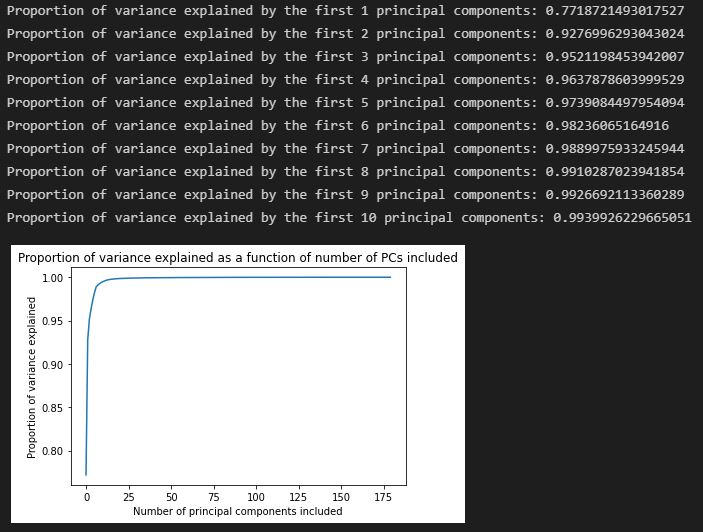
\includegraphics[width=0.9\textwidth]{Figures/Proportion_of_variance.JPG}
    \caption{Values for the first 10 proportions of variance, and the corrosponding graph}
\end{figure}

\noindent The proportion and the figure shows the context between the principal components and the ammount of
variance each iteration captures.

\newpage

\subsection{(b)}

\begin{minted}[linenos, bgcolor = bg]{python}
    # gets the fourth eigenvector
    e4 = PCevecs[:, 3] 
    # gets the fourth eigenvalue
    lambda4 = PCevals[3] 
    # In case the naming std is confusing -- 
    # the eigenvalues have a statistical interpretation
    # print(std4)
    std4 = np.sqrt(lambda4) 

    # Makes matrix filled with zeros
    diatoms_along_pc = np.zeros((7, 180))

    # Iterates the length of the matrix
    # For each row, add the mean diatom with added
    # values
    for i in range(7):
        diatoms_along_pc[i] = mean_diatom + ( e4 * std4 * (i-3))
        
    # Plotting each diatom
    for i in range(7):
        plot_diatom(diatoms_along_pc[i])

    plt.title('Diatom shape along PC1')
\end{minted}

\begin{figure}[H]
    \centering
    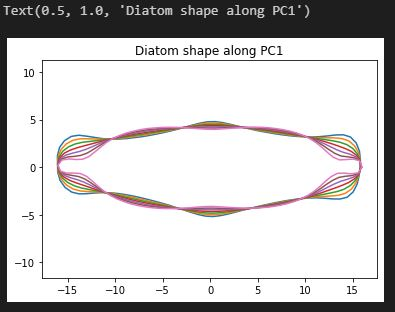
\includegraphics[width=0.75\textwidth]{Figures/Result_of_diatoms.JPG}
    \caption{Plotted diatom}
\end{figure}

